\chapter{Arhitektura i dizajn sustava}
	
		Arhitektura naše aplikacije može se intutivno podijeliti na prezentacijski, aplikacijski te podatkovni sloj. Njima redom odgovaraju idući podsustavi:
		\begin{itemize}
			\item 	Web aplikacija
			\item 	Web poslužitelj
			\item 	Baza podataka		
		\end{itemize}

		\begin{figure}[H]
			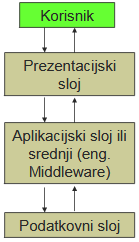
\includegraphics[scale=0.6]{slike/ArhitekturniPodsustavi.PNG}
			\centering
			\caption{Arhitektura sustava}
			\label{fig:arhitekturni_podsustavi}
		\end{figure}

		Kako bih se korisniku omogućilo korištenje naše aplikacije, korisnik na svojem uređaju (osobno računalo, laptop, mobitel ili tablet) mora koristiti \textit{web preglednik}, aplikaciju koja korištenjem stroja za vizualizaciju (u koji je uključen i interpreter JavaScript-a) omogućava
		pretvaranje koda naše web aplikacije (HTML, CSS i JavaScript) u vizualni multimedijski sadržaj.

		Za osnovnu komunikaciju s korisnikom koristi se \textit{web aplikacija}, program koji se pomoću HTTP (engl. \textit{Hyper Text Transfer Protocol}) protokola na zahtjev vraća korisnikovom web pregledniku. Web aplikacija služi kao sučelje između korisnika i poslovne logike aplikacije
		na web poslužitelju. Pomoću vizualnih komponenti korisniku se omogućava slanje HTTP zahtjeva na web poslužitelj te obrada i vizualizacija primljenih podataka u JSON (engl. \textit{JavaScript Object Notation}) formatu u ljudski razumljivom obliku.

		Primarni alat za komunikaciju s bazom podataka i za obradu poslovne logike je web poslužitelj kojem je omogućena komunikacija s web aplikacijom putem REST API (engl. \textit{Representational State Transfer Application Programming Interface}) tehnologije koja uvodi standardizirani način
		komunikacije s klijentom razmjenom JSON poruka. Na taj se način omogućava jasno određena i istovremeno fleksibilna razmjena podataka.

		Za izradu klijentske aplikacije izabrali smo jezik JavaScript zajedno s knjižnicom React koji omogućavaju jednostavnu i nativnu implementaciju arhitekture, zasnovane na događajima u klijentskom dijelu web aplikacije. Ovakav pristup omogućava dinamičko ažuriranje vizualnog prikaza na
		temelju korisničkih radnji i podataka, unesenih korisnikom. Kako bih se aplikacija mogla prikazati u korisnikovom web pregledniku, koristi se skupljač modula Webpack koji generira sve potrebne HTML, CSS i JavaScript datoteke koje se s poslužitelja šalju korisniku te se konačno prikazuju
		koristeći ugrađeni stroj za vizualizaciju web preglednika.

		Za opisivanje poslovne logike naše aplikacije odabrali smo programski jezik Java zajedno s radnim okvirom Spring Boot. Ovakav izbor tehnologija obrazložen je nativnom podrškom objektno usmjerenog pristupa programskim jezikom Java te jednostavnom implementacijom MVC 
		(engl. \textit{Model View Controller}) arhitekturnog modela u radnom okviru Spring Boot.

		MVC obrazac je stilistička varijacija arhitekture zasnovane na događajima koja se u našoj aplikaciji koristi kao alat za pojednostavljenje implementacije, testiranja i korištenja svih arhitekturnih podsustava. MVC obrazac dopušta paralelnu i neovisnu izradu tri komponente sustava
		na koje se intuitivno može podijeliti naša aplikacija:
		\begin{itemize}
			\item 	Model - Poslovna logika aplikacije koja definira i mijenja stanje koje aplikacija treba imati na temelju podataka iz kontrolera. 
			\item 	View - Vizualno sučelje ili korisnička strana aplikacije koja se koristi za vizualizaciju svih podataka unutar aplikacije, primarno dobivenih s web poslužitelja.
			\item 	Controller - Upravljački dio aplikacije koji komunikacijom s korisnikom kroz vizualni sloj ažurira stanje modela i/ili vizualnog stanja aplikacije.
		\end{itemize}

		\begin{figure}[H]
			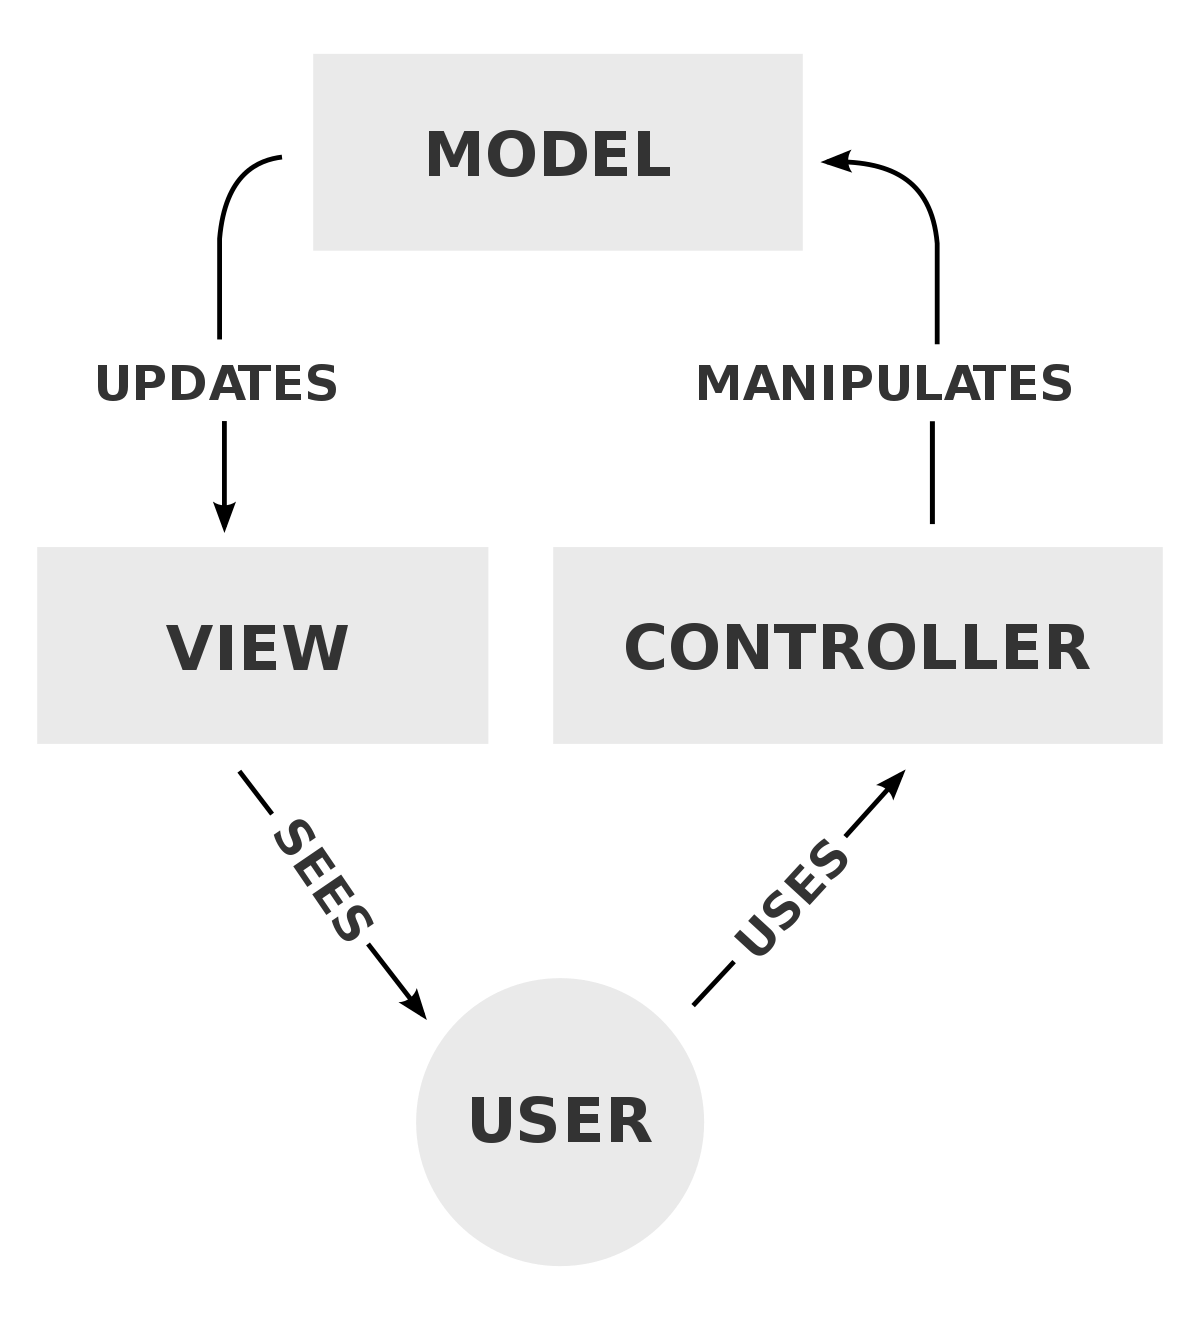
\includegraphics[scale=0.2]{slike/MVCObrazac.PNG}
			\centering
			\caption{MVC Obrazac}
			\label{fig:mvc_obrazac}
		\end{figure}

		\eject

				
		\section{Baza podataka}
			
			Za potrebe naseg sustava koristit ćemo sustav za upravljanje relacijskim bazama podataka MySQL.
   			Odlučili smo se koristiti ovaj sustav zbog toga što je softver otvorenog koda, ima izvrsnu potporu zajednice i jer je pouzdano i robusno rješenje.
			Glavna značajka relacijske baze podataka jest da se podaci organiziraju u tablice definirane svojim imenom i skupom atributa, a u shemi baze podataka se definira kako se 				pospremaju podaci i povezuju tablice.
   			Zadaća baze podataka je brza i jednostavna pohrana, izmjena i dohvat podataka za daljnju obradu.
			Baza podataka ove aplikacije sastoji se od sljedecih entiteta: 
			\begin{itemize}
				\item Korisnik
				\item Članak
				\item Komentar
				\item Ocjena
				\item Notifikacija
			  \end{itemize}
		
			\subsection{Opis tablica}
			

				\textbf{Korisnik} Ovaj entitet sadržava sve važne informacije o korisniku aplikacije.
				Sadrži atribute: id, ime, prezime, email, uloga, lozinka i potvrđen. Ovaj entitet u vezi je
				One-to-Many s entitetom Članak preko atributa id korisnika, u vezi One-to-Many s entitetom Komentar preko atributa id korisnika,
				te u dvostrukoj One-to-Many vezi s entitetom Notifikacija preko atributa id korisnika.
				
				
				
				\begin{longtblr}[
					label=none,
					entry=none
					]{
						width = \textwidth,
						colspec={|X[6,l]|X[6, l]|X[20, l]|}, 
						rowhead = 1,
					} %definicija širine tablice, širine stupaca, poravnanje i broja redaka naslova tablice
					\hline \SetCell[c=3]{c}{\textbf{Korisnik}}	 \\ \hline[3pt]
					\SetCell{LightGreen}id & BIGINT	& jedinstveni brojčani identifikator 	\\ \hline
					Ime	& VARCHAR &  ime korisnika 	\\ \hline 
					Prezime & VARCHAR & prezime korisnika  \\ \hline 
					Email & VARCHAR	&  	e-mail adresa korisnika	\\ \hline 
					Uloga & TINYINT	&  	oznaka razine privilegije korisnika (korisnik, moderator, administrator)	\\ \hline 
					Lozinka & VARCHAR	&  	hash lozinke	\\ \hline 
					Potvrđen & BOOL	&  	oznaka da je korisnik potvrdio e-mail adresu	\\ \hline 
				\end{longtblr}

				
				\textbf{Članak} Ovaj entitet sadržava sve važne informacije vezane za pospremljene članke.
				Sadrži atribute: id, autorid, naslov, sadržaj, objavljen, datumobjave, tagovi i moderiran. Ovaj entitet u vezi je
				Many-to-One s entitetom Korisnik preko atributa autorid, u vezi One-to-Many s entitetom Komentar preko atributa id članka,
				te u One-to-Many vezi s entitetom Ocjena preko atributa id članka.
				

				\begin{longtblr}[
					label=none,
					entry=none
					]{
						width = \textwidth,
						colspec={|X[6,l]|X[6, l]|X[20, l]|}, 
						rowhead = 1,
					} %definicija širine tablice, širine stupaca, poravnanje i broja redaka naslova tablice
					\hline \SetCell[c=3]{c}{\textbf{Članak}}	 \\ \hline[3pt]
					\SetCell{LightGreen}id & BIGINT	& jedinstveni brojčani identifikator  	\\ \hline
					\SetCell{LightBlue} autorid	& BIGINT &   jedinstveni brojčani identifikator autora (korisnik.id)	\\ \hline 
					Naslov & VARCHAR &  naslov članka  \\ \hline 
					Sadržaj & TEXT	&  	tekst članka	\\ \hline 
					Objavljen & BOOL	&  	oznaka da je članak javno dostupan	\\ \hline 
					DatumObjave & DATETIME	&  	datum i vrijeme objave članka	\\ \hline 
					Tagovi & VARCHAR	&  	popis tagova prema kojima se može pronaći članak	\\ \hline 
					Moderiran & BOOL	&  	oznaka da je članak pregledao moderator	\\ \hline 
				\end{longtblr}

				\textbf{Komentar} Ovaj entitet sadržava sve važne informacije vezane za komentare na članke.
				Sadrži atribute: id, autorid, članakid, sadržaj, vidljivost i datumobjave. Ovaj entitet u vezi je
				Many-to-One s entitetom Korisnik preko atributa autorid te u vezi Many-to-One s entitetom Članak preko atributa članakid.
				

				\begin{longtblr}[
					label=none,
					entry=none
					]{
						width = \textwidth,
						colspec={|X[6,l]|X[6, l]|X[20, l]|}, 
						rowhead = 1,
					} %definicija širine tablice, širine stupaca, poravnanje i broja redaka naslova tablice
					\hline \SetCell[c=3]{c}{\textbf{Komentar}}	 \\ \hline[3pt]
					\SetCell{LightGreen}id & BIGINT	& jedinstveni brojčani identifikator  	\\ \hline
					\SetCell{LightBlue} autorid	& BIGINT &   jedinstveni brojčani identifikator autora (korisnik.id)	\\ \hline 
					\SetCell{LightBlue} članakid	& BIGINT &   jedinstveni brojčani identifikator članka (članak.id)	\\ \hline 
					Sadržaj & TEXT	&  	tekst komentara	\\ \hline 
					Vidljivost & BOOL	&  	oznaka da je komentar javno dostupan	\\ \hline 
					DatumObjave & DATETIME	&  	datum i vrijeme objave komentara	\\ \hline 
				\end{longtblr}
				
				\textbf{Ocjena} Ovaj entitet sadržava sve važne informacije vezane za ocjene članaka.
				Sadrži atribute: id, članakid, ocjena. Ovaj entitet u vezi u vezi Many-to-One s entitetom Članak preko atributa članakid.
				
				
				\begin{longtblr}[
					label=none,
					entry=none
					]{
						width = \textwidth,
						colspec={|X[6,l]|X[6, l]|X[20, l]|}, 
						rowhead = 1,
					} %definicija širine tablice, širine stupaca, poravnanje i broja redaka naslova tablice
					\hline \SetCell[c=3]{c}{\textbf{Ocjena}}	 \\ \hline[3pt]
					\SetCell{LightGreen}id & BIGINT	&  jedinstveni brojčani identifikator 	\\ \hline
					\SetCell{LightBlue} članakid	& BIGINT &   jedinstveni brojčani identifikator članka (članak.id)	\\ \hline 
					Ocjena & TINYINT	&  	ocjena članka (cijeli broj od 1 do 5)	\\ \hline 
				\end{longtblr}

				
				\textbf{Notifikacija} Ovaj entitet sadržava sve važne informacije vezane za komentare na članke.
				Sadrži atribute: id, idpošiljatelj, idprimatelj, prioritet, naslov i sadržaj. Ovaj entitet je u dvostrukoj vezi
				Many-to-One s entitetom Korisnik preko atributa idpošiljatelj i idprimatelj.
				

				
				\begin{longtblr}[
					label=none,
					entry=none
					]{
						width = \textwidth,
						colspec={|X[6,l]|X[6, l]|X[20, l]|}, 
						rowhead = 1,
					} %definicija širine tablice, širine stupaca, poravnanje i broja redaka naslova tablice
					\hline \SetCell[c=3]{c}{\textbf{Notifikacija}}	 \\ \hline[3pt]
					\SetCell{LightGreen}id & BIGINT	&  jedinstveni brojčani identifikator 	\\ \hline
					\SetCell{LightBlue} idpošiljatelj	& BIGINT &   jedinstveni brojčani identifikator pošiljatelja (korisnik.id)	\\ \hline 
					\SetCell{LightBlue} idprimatelj	& BIGINT &   jedinstveni brojčani identifikator primatelja (korisnik.id)	\\ \hline 
					Prioritet & TINYINT	&  	oznaka prioriteta poruke	\\ \hline 
					Naslov & VARCHAR	&  	naslov poruke	\\ \hline 
					Sadržaj & TEXT	&  	tekst poruke	\\ \hline 
				\end{longtblr}
				
				
			
			\subsection{Dijagram baze podataka}
					\begin{figure}[H]
					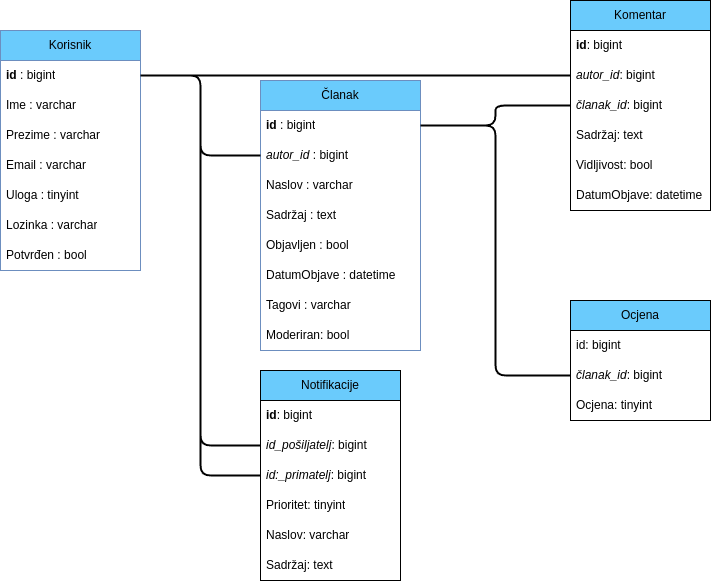
\includegraphics[scale=0.5]{slike/baza.png}
					\centering
					\caption{E-R dijagram baze podataka}
					\label{fig:baza}
				\end{figure}
		
			\eject
			
			
		\section{Dijagram razreda}
		
			Slike od 4.4 - 4.9 prikazuju razrede koji pripadaju backend dijelu MVC arhitekture. Slika 4.4 prikazuje controller razrede koji definiraju pristupne točke i ponašanje za svaku. 
			Osim toga manipuliraju DTO(Data transfer object), koji su definirani u paketu dto prikazan na slici 4.5 koji je podijeljen u request i response podpakete. 
			Metode implementirane u controller razredima vraćaju JSON u tijelu te odgovarajući HTTP status kod. 
			Logika ponašanja za svaku pristupnu točku definirana je u service razredima koje implementiraju pripadna service sučelja, a prikazani su na slici 4.6. 
			Zbog lakše organizacije service razredi su podijeljeni po funkcionalnosti. Oni pomoću repository sučelja koja nasljeđuju JpaRepository (prikazana na slici 4.7) komuniciraju s bazom podataka.  
			JpaRepository repository parametriziran je odgovarajućom klasom iz paketa enttiy (Slika 4.8) koje opisuju model baze. Za autentifikaciju korisnika koriste se metode implementirane u razredima paketa jwt prikazane na slici 4.9.
			
			\eject

			\begin{figure}[H]
				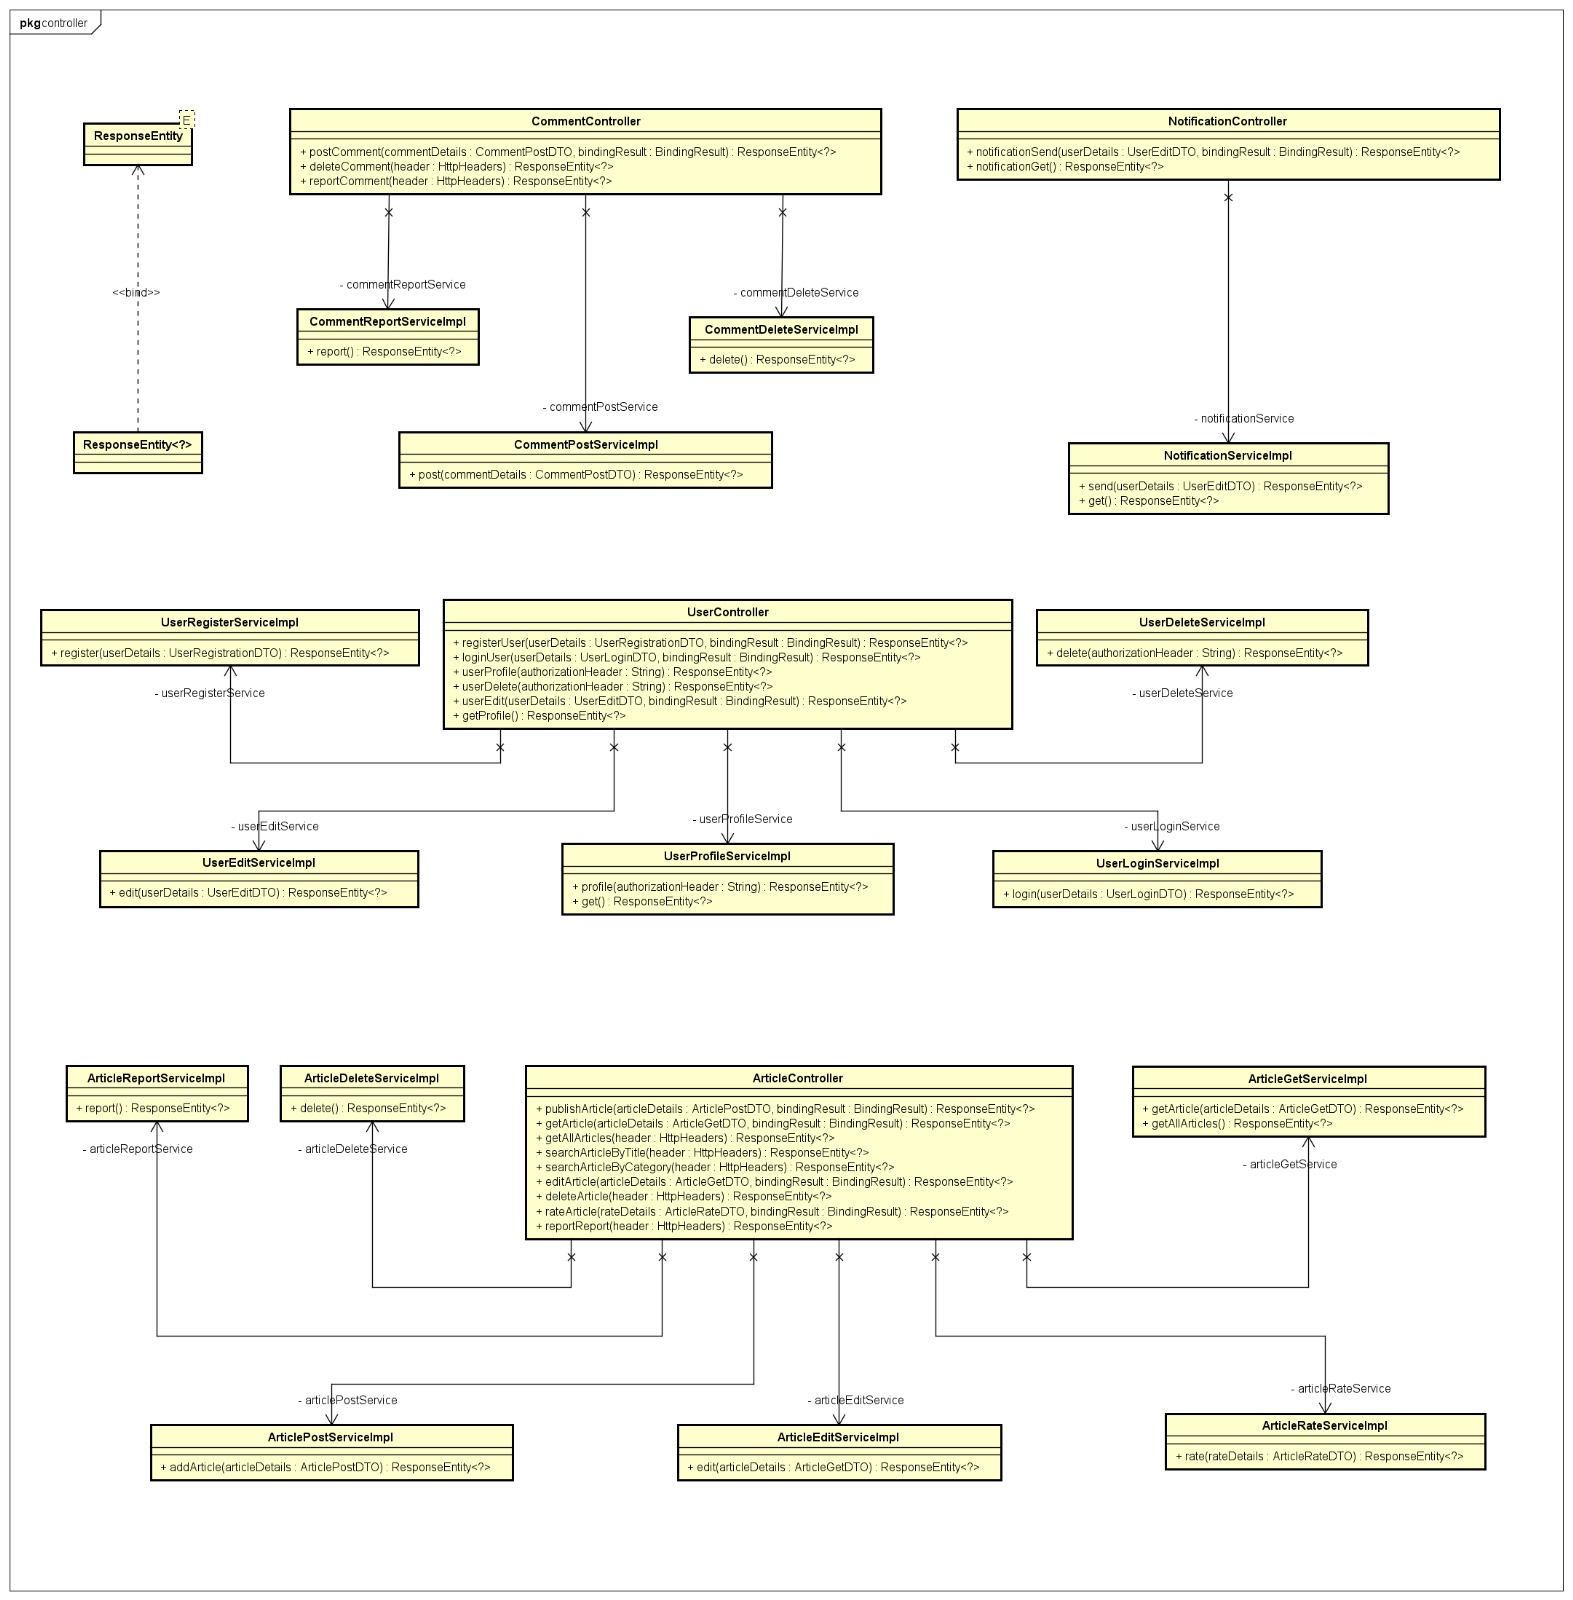
\includegraphics[scale=0.4]{slike/DijagramRazreda1.jpg}
				\centering
				\caption{Dijagram razreda - dio Controllers}
				\label{fig:class_diagram_controllers}
			\end{figure}

			\eject

			\begin{figure}[H]
				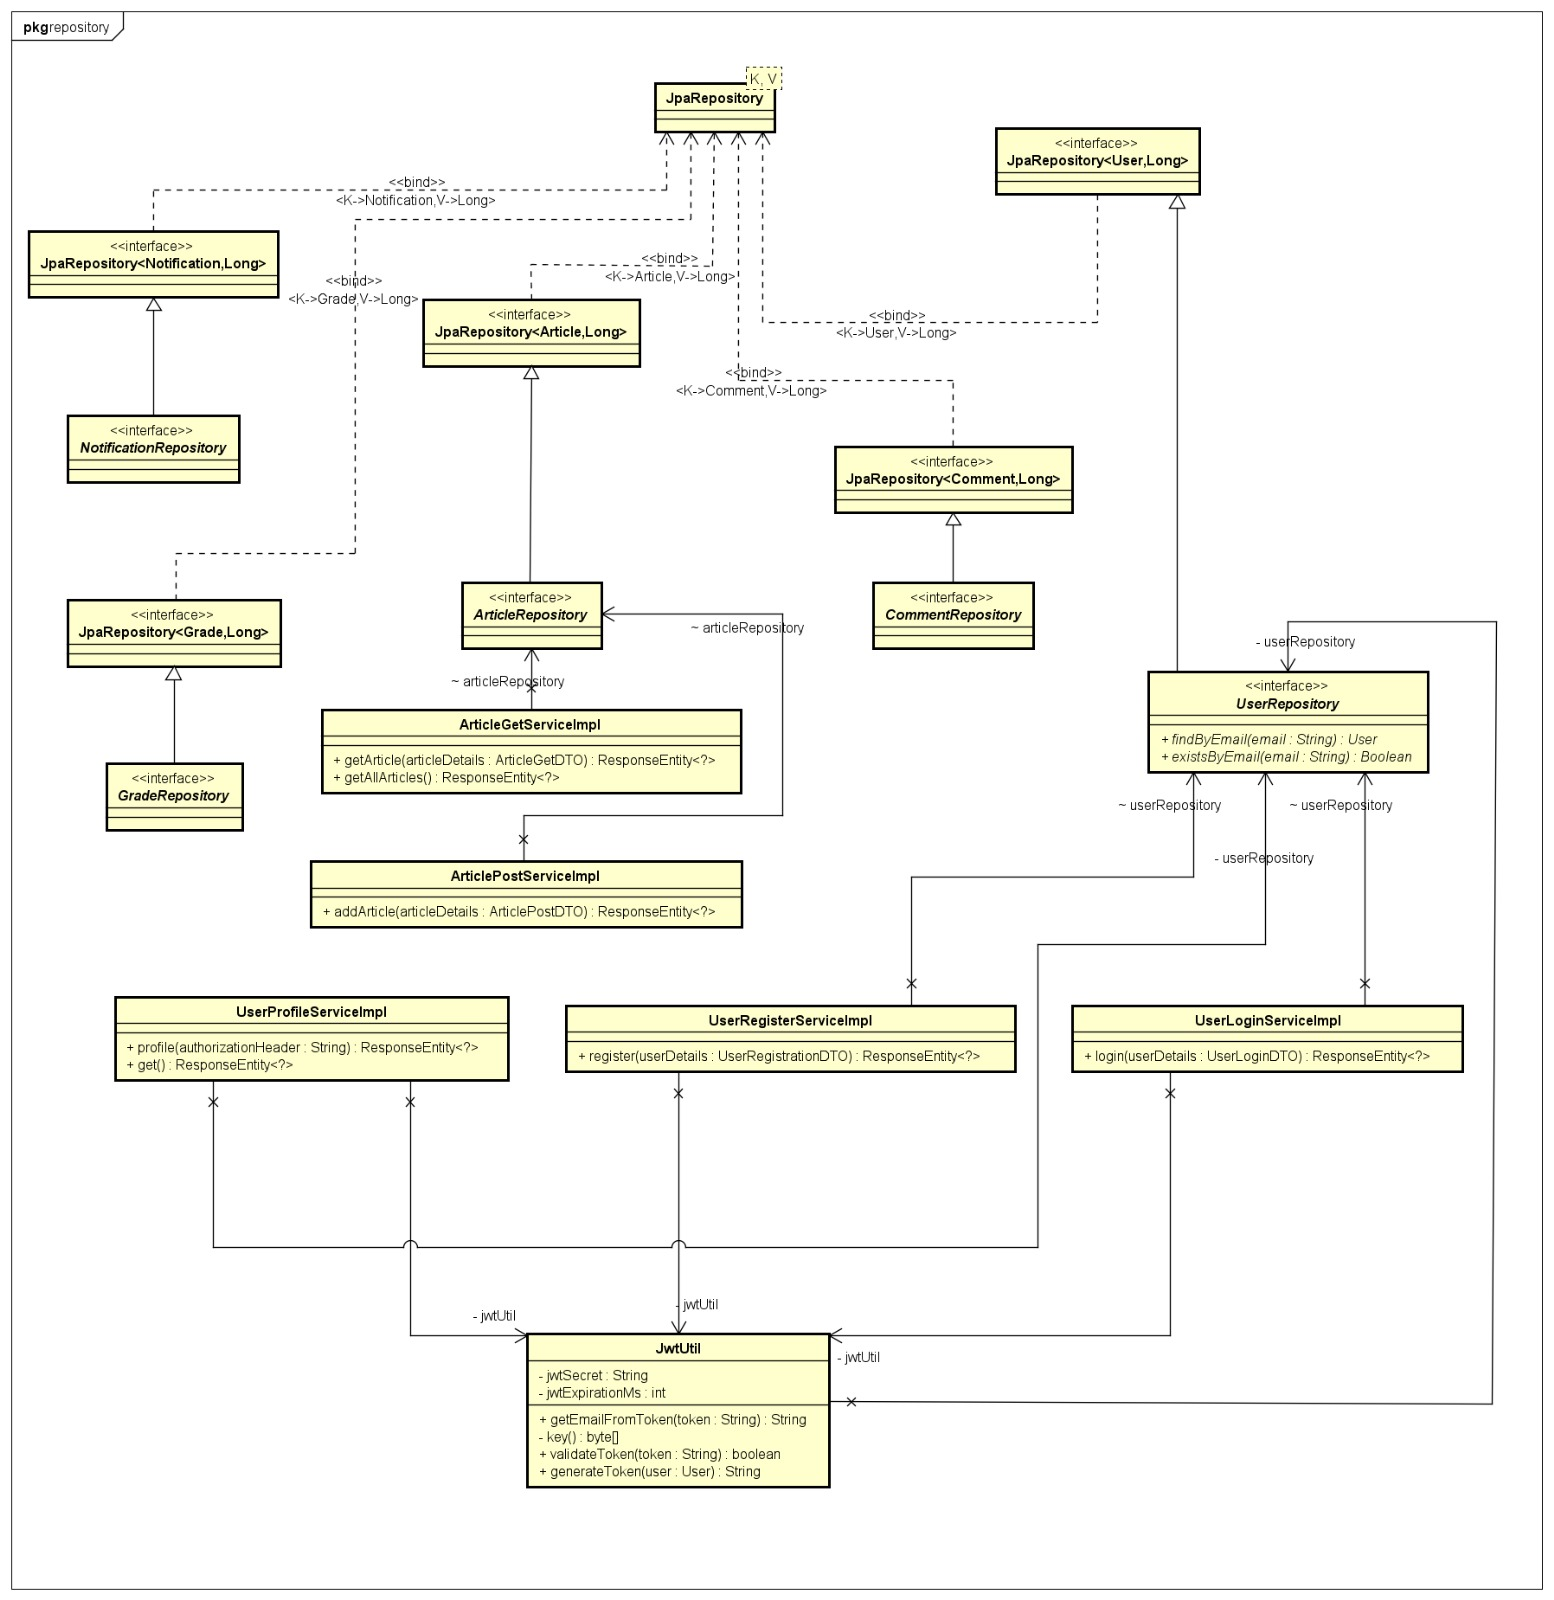
\includegraphics[scale=0.4]{slike/DijagramRazreda2.jpg}
				\centering
				\caption{Dijagram razreda - dio DTO}
				\label{fig:class_diagram_dto}
			\end{figure}

			\eject

			\begin{figure}[H]
				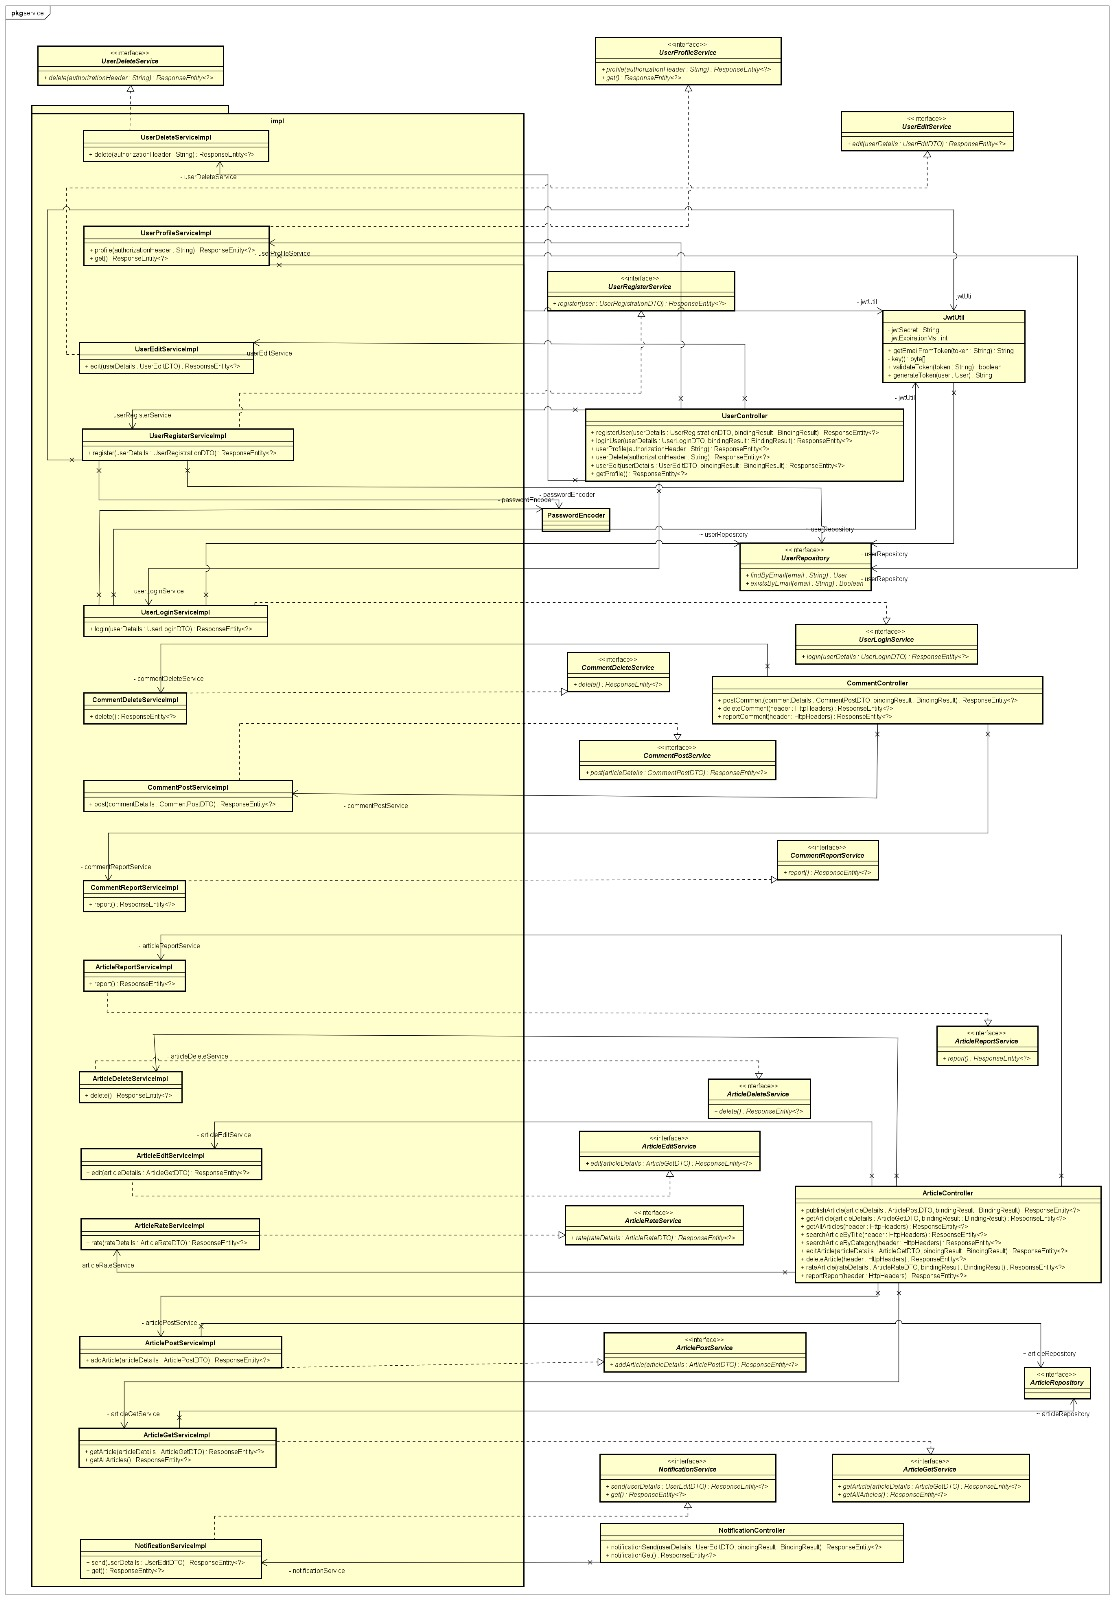
\includegraphics[scale=0.5]{slike/DijagramRazreda3.jpg}
				\centering
				\caption{Dijagram razreda - dio Service}
				\label{fig:class_diagram_service}
			\end{figure}

			\eject

			\begin{figure}[H]
				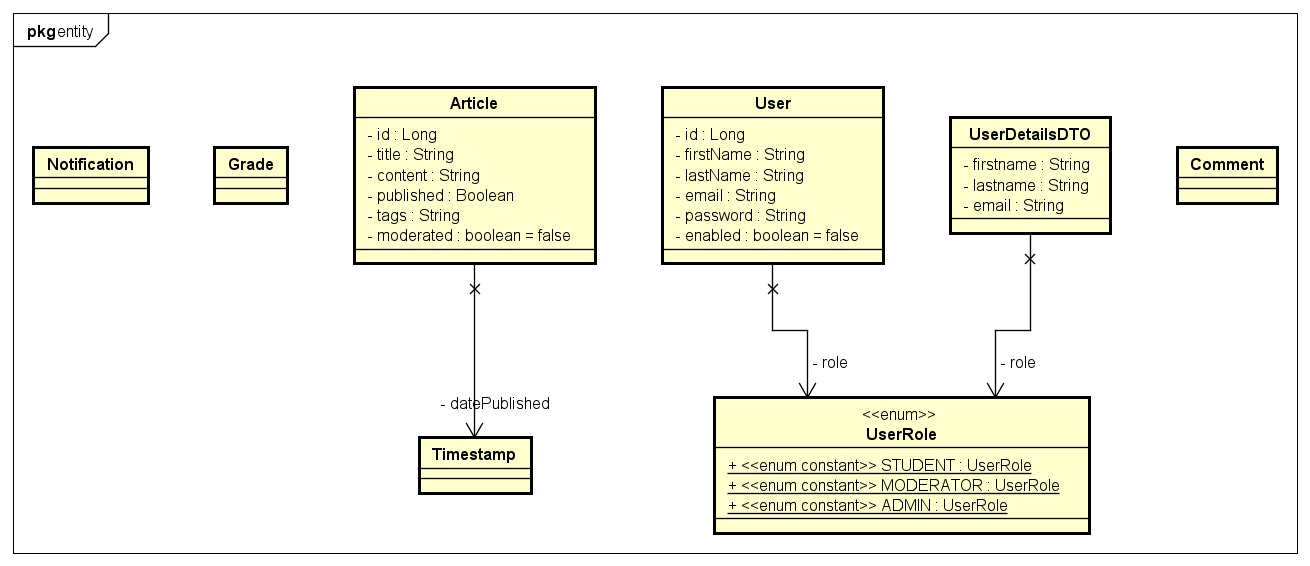
\includegraphics[scale=0.4]{slike/DijagramRazreda4.jpg}
				\centering
				\caption{Dijagram razreda - dio Repository}
				\label{fig:class_diagram_repository}
			\end{figure}

			\begin{figure}[H]
				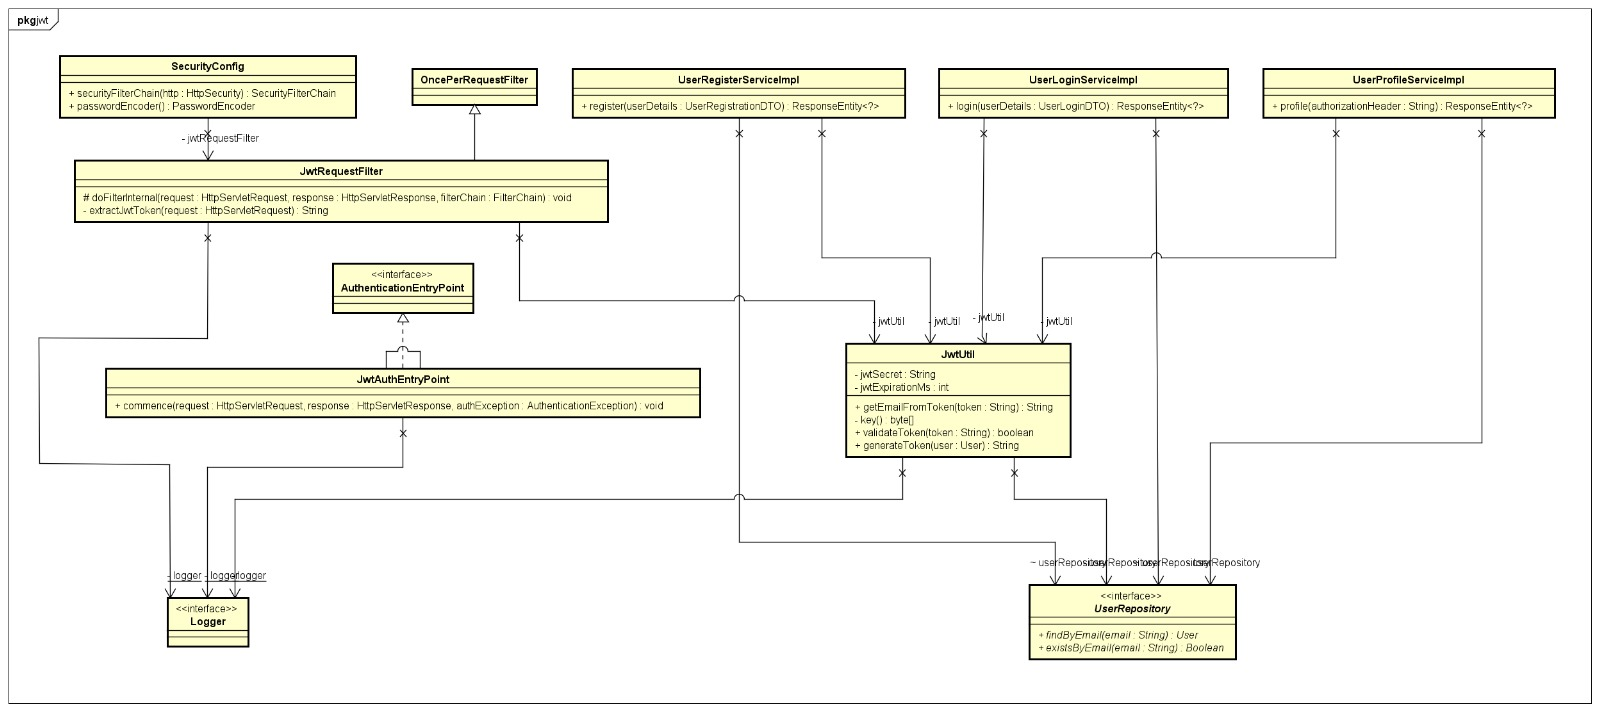
\includegraphics[scale=0.4]{slike/DijagramRazreda5.jpg}
				\centering
				\caption{Dijagram razreda - dio Entity}
				\label{fig:class_diagram_entity}
			\end{figure}

			\eject

			\begin{figure}[H]
				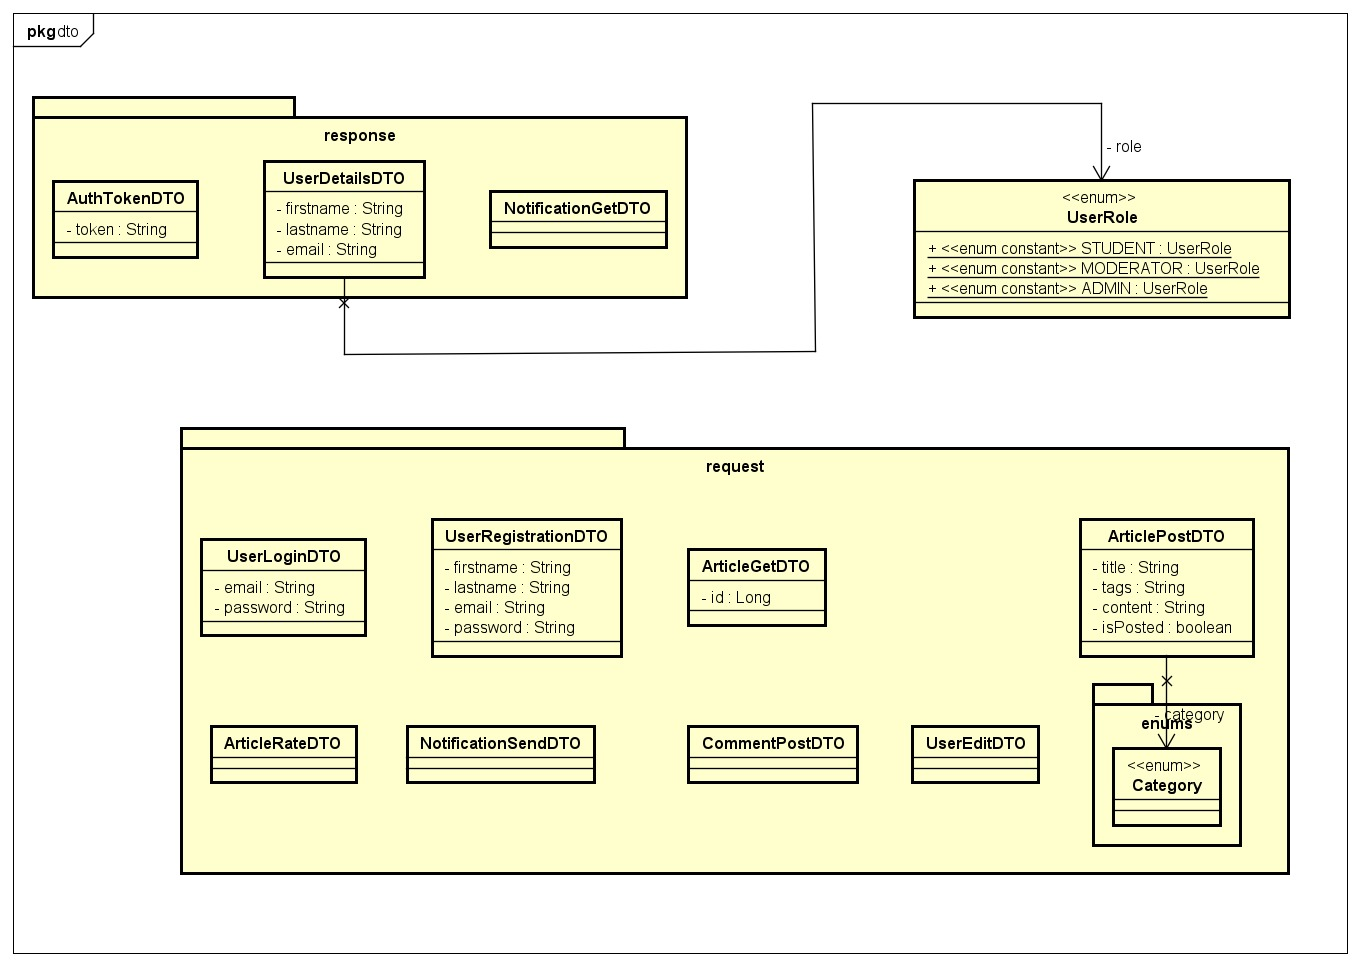
\includegraphics[scale=0.4]{slike/DijagramRazreda6.jpg}
				\centering
				\caption{Dijagram razreda - dio JWT}
				\label{fig:class_diagram_jwt}
			\end{figure}

			\eject

			% \textbf{\textit{dio 2. revizije}}\\			
			
			% \textit{Prilikom druge predaje projekta dijagram razreda i opisi moraju odgovarati stvarnom stanju implementacije}
			
			
			
			% \eject
		
		% \section{Dijagram stanja}
			
			
		% 	\textbf{\textit{dio 2. revizije}}\\
			
		% 	\textit{Potrebno je priložiti dijagram stanja i opisati ga. Dovoljan je jedan dijagram stanja koji prikazuje \textbf{značajan dio funkcionalnosti} sustava. Na primjer, stanja korisničkog sučelja i tijek korištenja neke ključne funkcionalnosti jesu značajan dio sustava, a registracija i prijava nisu. }
			
			
		% 	\eject 
		
		% \section{Dijagram aktivnosti}
			
		% 	\textbf{\textit{dio 2. revizije}}\\
			
		% 	 \textit{Potrebno je priložiti dijagram aktivnosti s pripadajućim opisom. Dijagram aktivnosti treba prikazivati značajan dio sustava.}
			
		% 	\eject
		% \section{Dijagram komponenti}
		
		% 	\textbf{\textit{dio 2. revizije}}\\
		
		% 	 \textit{Potrebno je priložiti dijagram komponenti s pripadajućim opisom. Dijagram komponenti treba prikazivati strukturu cijele aplikacije.}
